\chapter{Resultados}
\section*{Introducci'on}
\addcontentsline{toc}{section}{Introducci'on}

En 'este cap'itulo se describir'an los resultados obtenidos en modelado y simulaci'on del centro de datos en CloudSim. La experimentaci'on fue desarrollada en una computadora con  un procesador Intel Core i5  con la siguiente configuraci'on: 2.5 GHz, 3 MB de cach'e, 4 GB de RAM , Linux Ubuntu 14.04 lts 64 bits como sistema operativo y JDK 8.6.

Para evaluar los algoritmos de calendarizaci'on seleccionados se ha implementado un entorno de c'omputo en la nube que consiste en un datacenter, un broker, m'aquinas virtuales y host.  Con el objetivo de evaluar el tiempo de ejecuci'on y el costo de procesamiento en el datacenter tras ejecutar ciertos n'umero de tareas (cloudlets).

Para la configuraci'on del centro de datos en CloudSim se utilizaron diez host, cinco m'aquinas virtuales por host y las tareas fueron establecidas en un intervalo de 100 – 500 (tabla 3.1).
Como se puede apreciar en la tabla 3.2, cada host tuvo 2048 Mb de memoria RAM, Dos n'ucleos de procesamiento, de almacenamiento de 800 GB o 1TB elegidas de manera aleatoria, el ancho de banda fue de 1GB/s.


\begin{table}[]
	\centering
	\caption{Configuraci'on Datacenter, Fuente: Elaboraci'on propia.}
	\label{my-label}
	\begin{tabular}{@{}cc@{}}
		\toprule
		\multicolumn{2}{c}{{\bf Datacenter}} \\ \midrule
		Host              & 10               \\
		VM                & 5                \\
		Cloudlet          & 100-500          \\ \bottomrule
	\end{tabular}
\end{table}

\begin{table}[]
	\centering
	\caption{Configuraci'on de Host, Fuente: Elaboraci'on propia.}
	\label{my-label}
	\begin{tabular}{@{}cc@{}}
		\toprule
		\multicolumn{2}{c}{{\bf Host}} \\ \midrule
		RAM           & 2048 MB        \\
		CPU           & 2              \\
		Storage       & 800GB-1TB      \\ \midrule
		BW            & 1 GB/s        
	\end{tabular}
\end{table}

En la tabla 3.3 se muestran los par'ametros que se consider'o para las m'aquinas virtuales, donde cada VM tendr'a 10 GB de almacenamiento, 512 MB  o 1 GB seleccionado de manera aleatoria, adem'as para la caracter'istica del procesador se tiene  la propiedad MIPS (million instructions per second) con 250 o 500 y un ancho de banda de 1000kb/s.


\begin{table}[]
	\centering
	\caption{Virtual Machine, Fuente: Elaboraci'on propia.}
	\label{my-label}
	\begin{tabular}{@{}cc@{}}
		\toprule
		\multicolumn{2}{c}{{\bf VirtualMachine}} \\ \midrule
		RAM               & 512 MB| 1GB          \\
		MIPS              & 250 | 500            \\
		Storage           & 10 GB                \\ \midrule
		BW                & 1 GB/s              
	\end{tabular}
\end{table}


Para la configuraci'on de las tareas, se tom'o el tama'no con un intervalo de 1kb a 10kb,  el par'ametro fileSize que representa el tama'no del archivo de entrada va de 300b a 1.8kb as'i como el archivo de salida, como par'ametro final se tiene los MIPS que ir'an de 1 a 3.



\begin{table}[]
	\centering
	\caption{Configuraci'on Cloudlet, Fuente: Elaboraci'on propia.}
	\label{my-label}
	\begin{tabular}{@{}cc@{}}
		\toprule
		\multicolumn{2}{c}{{\bf Cloudlet}} \\ \midrule
		length           & 1kb-10kb        \\
		MIPSlength       & 300b-1.8kb      \\
		length           & 300b-1.8kb      \\ \midrule
		length           & 1000 kb/s      
	\end{tabular}
\end{table}

\begin{figure}
	\caption{Promedio tiempo de ejecuci'on con tareas 100-500, Fuente: Elaboraci'on propia.}
	\centering
	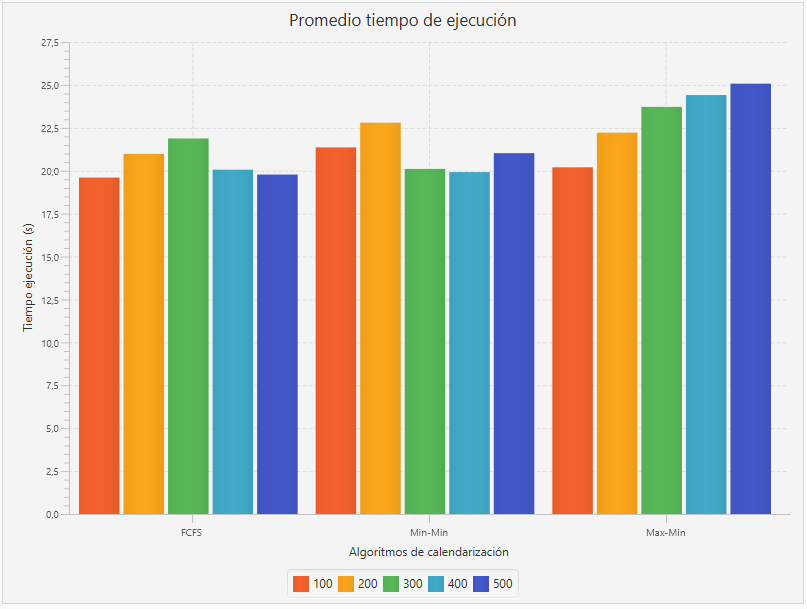
\includegraphics[scale=0.5]{media/tiempoejecucion}
\end{figure}

En la figura 3.1, se puede observar el promedio del tiempo de ejecuci'on en ms para diferentes cantidades de tareas (de 100 a 500). A primera vista con el algoritmo FCFS y Min-Min se mantiene un tiempo de ejecuci'on sin muchos cambios a pesar del aumento en la carga de tareas, a diferencia del algoritmo Max-Min que aument'o el tiempo de ejecuci'on a medida que se increment'o el n'umero de tareas.

\begin{figure}
	\caption{Promedio costo de procesamiento con tareas 100-500, Fuente: Elaboraci'on propia.}
	\centering
	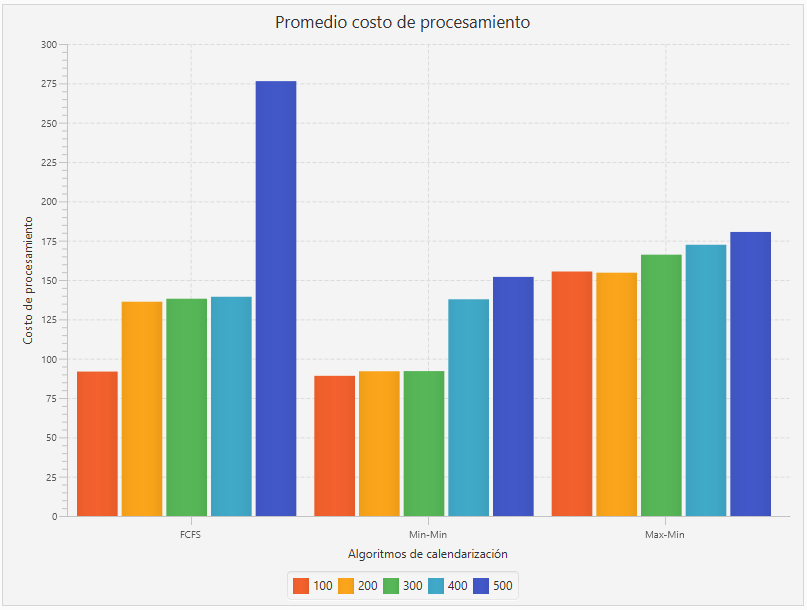
\includegraphics[scale=0.5]{media/costoproce}
\end{figure}

\newpage
El costo de procesamiento de acuerdo a cada algoritmo se puede observar en la figura 3.2, en donde el algoritmo FCFS tiene un incremento dr'astico al realizar la prueba con 500 tareas. El algoritmo Max-Min se conserv'o sin muchos cambios a pasar de los cambios en la cantidad de tareas, mientras que Min-Min tiene un menor costo de procesamiento cuando las tareas son inferiores a 300.

\begin{figure}
	\caption{Tiempo ejecuci'on 50 muestras FCFS, Fuente: Elaboraci'on propia}
	\centering
	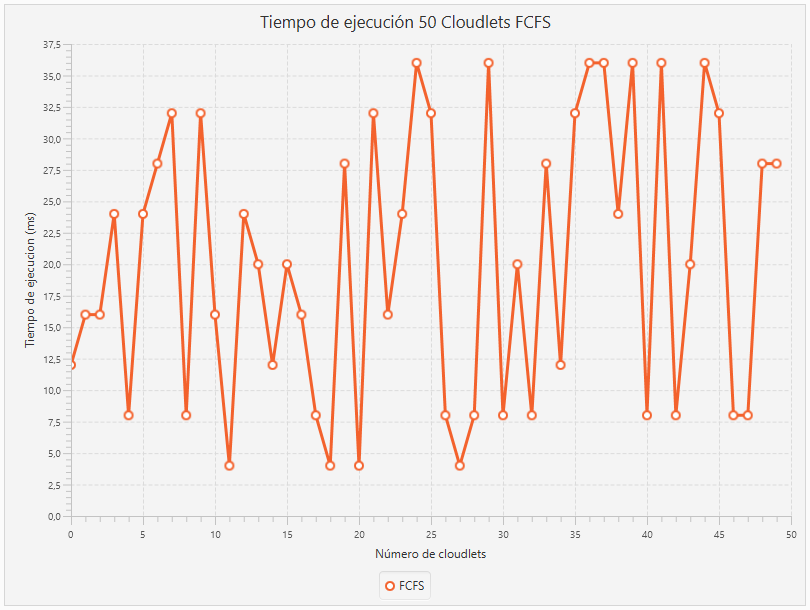
\includegraphics[scale=0.5]{media/fcfs}
\end{figure}

\bigskip
Para mostrar el comportamiento del tiempo de ejecuci'on por cada algoritmo, se tomaron 50 muestras de una simulaci'on de 500 tareas. En la figura 3.3, se puede apreciar que el algoritmo FCFS tiene un comportamiento inestable ya que algunas tareas pueden tener menor complejidad o tama'no, lo que implica una respuesta r'apida.

\begin{figure}
	\caption{Tiempo ejecuci'on 50 muestras Max-Min, Fuente: Elaboraci'on propia}
	\centering
	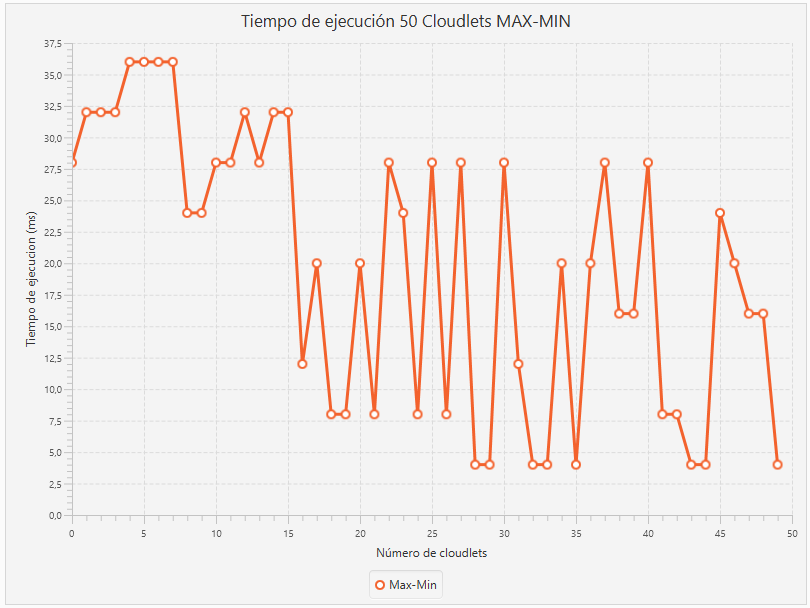
\includegraphics[scale=0.5]{media/max-min}
\end{figure}

\bigskip
 En la figura 3.4 se tiene la misma simulaci'on pero con el algoritmo Max-Min, de acuerdo a las caracter'isticas de este calendarizador, en las primeras tareas se toma un mayor tiempo en responder y va disminuyendo de manera gradual, sin embargo a'un es inestable en las 'ultimas muestras ya que no se contempla el grado de complejidad es decir el par'ametro MIPS de los cloudlets.

\begin{figure}
	\caption{Tiempo ejecuci'on 50 muestras Min-Min, Fuente: Elaboraci'on propia}
	\centering
	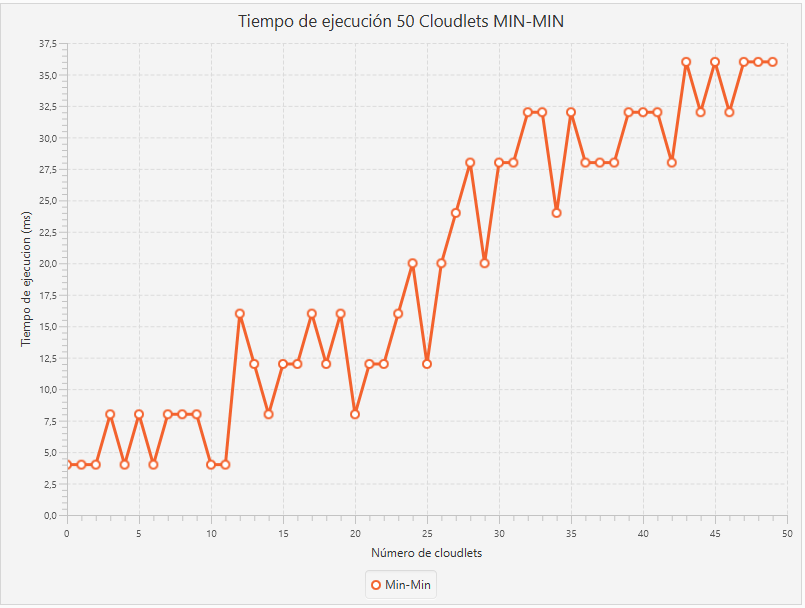
\includegraphics[scale=0.5]{media/min-min}
\end{figure}

\bigskip
Por 'ultimo tenemos el algoritmo Min-Min en el que el tiempo de ejecuci'on fue aumentando conforme se resolv'ian las tareas (figura 3.6).

\begin{table}[]
	\centering
	\caption{Desviaci'on est'andar del tiempo de ejecuci'on, Fuente: Elaboraci'on propia}
	\label{my-label}
	\begin{tabular}{@{}cc@{}}
		\toprule
		{\bf Algoritmo} & \multicolumn{1}{l}{{\bf Desviaci'on est'andar}} \\ \midrule
		FCFS & 11.00619 \\
		MAX-MIN & 8.91444 \\
		MIN-MIN & 11.25613 \\ \bottomrule
	\end{tabular}
\end{table}

Observando la desviaci'on est'andar de 'estas muestras anteriores, el algoritmo Min-Min y FCFS tuvieron m'as variaciones en las muestras con respecto a la media, mientras que el Max-Min tuvo las variaciones por debajo de las dos anteriores (Cuadro 3.5).